%!TEX program=xelatex
%!TEX program=bibtex
%!TEX program=xelatex
%!TEX program=xelatex
% !Mode:: "TeX:UTF-8"
\documentclass{article}
\usepackage[utf8]{inputenc}
\usepackage{pgfplots}
\usepackage{tikz-dependency}
\usepackage{graphicx}
\usepackage{tikz}
\usepgflibrary{arrows.meta}
\usetikzlibrary{fit}
\usepackage{pgfplots}
\usepackage{times}
\usepackage{latexsym}
\usepackage{caption}
\thispagestyle{empty}
\pgfplotsset{compat=1.9}

\begin{document}
\begin{figure}[htb]
    \centering
    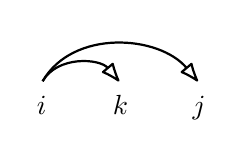
\begin{tikzpicture}[
        dep arrow/.style={
        arrows = {-Latex[round,open,length=8pt,width=6pt]},
        thick
        },
        dot/.style={
                inner sep=0pt,
                circle,
                draw=none
            },
        label/.style={
                anchor=base,
            }]
        \node [dot] (i) {};
        \node [dot] (k) at ($(i) + (1cm, 0)$) {};
        \node [dot] (j) at ($(k) + (1cm, 0)$) {};

        \node [label] at ($(i) + (0, -0.4cm)$) {$i$};
        \node [label] at ($(k) + (0, -0.4cm)$) {$k$};
        \node [label] at ($(j) + (0, -0.4cm)$) {$j$};

        \draw [dep arrow] [out=60,in=130] (i) to (k);
        \draw [dep arrow] [out=60,in=130] (i) to (j);
    \end{tikzpicture}
\end{figure}
\end{document}
